\documentclass[12pt]{report}
\usepackage{%
	amsfonts,%
	amsmath,%	
	amssymb,%
	amsthm,%
	algorithm,%
	babel,%
	bbm,%
	etex,%
	%biblatex,%
	caption,%
	centernot,%
	color,%
	dsfont,%
	enumerate,%
	epsfig,%
	epstopdf,%
	geometry,%
	graphicx,%
	hyperref,%
	latexsym,%
	mathtools,%
	multicol,%
	pgf,%
	pgfplots,%
	pgfplotstable,%
	pgfpages,%
	proof,%
	psfrag,%
	subfigure,%	
	tikz,%
	ulem,%
	url%
}	
\usepackage[noend]{algpseudocode}
\usepackage[mathscr]{eucal}
\usepgflibrary{shapes}
\usetikzlibrary{%
  	arrows,%
	backgrounds,%
	chains,%
	decorations.pathmorphing,% /pgf/decoration/random steps | erste Graphik
	decorations.text,%
	matrix,%
  	positioning,% wg. " of "
  	fit,%
	patterns,%
  	petri,%
	plotmarks,%
  	scopes,%
	shadows,%
  	shapes.misc,% wg. rounded rectangle
  	shapes.arrows,%
	shapes.callouts,%
  	shapes%
}

\theoremstyle{plain}
\newtheorem{thm}{Theorem}[section]
\newtheorem{lem}[thm]{Lemma}
\newtheorem{prop}[thm]{Proposition}
\newtheorem{cor}[thm]{Corollary}

\theoremstyle{definition}
\newtheorem{defn}[thm]{Definition}
\newtheorem{conj}[thm]{Conjecture}
\newtheorem{exmp}[thm]{Example}
\newtheorem{assum}[thm]{Assumptions}
\newtheorem{axiom}[thm]{Axiom}

\theoremstyle{remark}
\newtheorem{rem}{Remark}
\newtheorem{note}{Note}
\newtheorem{fact}{Fact}

\newcommand{\norm}[1]{\left\lVert#1\right\rVert}
\newcommand{\indep}{\!\perp\!\!\!\perp}
\DeclarePairedDelimiter\abs{\lvert}{\rvert}%
\newcommand\numberthis{\addtocounter{equation}{1}\tag{\theequation}}
\newcommand{\tr}{\operatorname{tr}}
\newcommand{\R}{\mathbb{R}}
\newcommand{\N}{\mathbb{N}}
\newcommand{\E}{\mathbb{E}}
\newcommand{\Z}{\mathbb{Z}}
\newcommand{\B}{\mathscr{B}}
\newcommand{\C}{\mathcal{C}}
\newcommand{\T}{\mathscr{T}}
\newcommand{\F}{\mathcal{F}}
\newcommand{\G}{\mathcal{G}}
%\newcommand{\ba}{\begin{align*}}
%\newcommand{\ea}{\end{align*}}
\DeclareMathOperator*{\argmax}{arg\,max}
\renewcommand{\qedsymbol}{$\blacksquare$}
\makeatletter
\def\BState{\State\hskip-\ALG@thistlm}
\makeatother

\makeatletter
\def\th@plain{%
  \thm@notefont{}% same as heading font
  \itshape % body font
}
\def\th@definition{%
  \thm@notefont{}% same as heading font
  \normalfont % body font
}
\makeatother
\date{}
\usepackage{scribe_e1244}
\usepackage{times}
\begin{document}
\lecturer{Aditya Gopalan, Parimal Parag}		
\scribe{VINAY SIRAM,S HEMANTH}					
\lecturenumber{6}						
\lecturedate{January 19}					
\maketitle
\section{Recap}
{\bf Neyman-Pearson framework for binary hypothesis testing: }
\begin{align*}
H_0 : Y \sim \mathbb{P}_0  \text{ on   } \Gamma \\ 
H_1 : Y \sim \mathbb{P}_1   \text{on   } \Gamma \\[-10pt]
\end{align*}
For given $\alpha$ $\in$ [0,1] Neyman-Pearson problem is to find $\delta$ that maximizes 
$P_D$($\delta$) s.t $P_F(\delta)$ $\leq$ $\alpha$\\
where $P_D$($\delta$) = $\mathbb{E}_1$[$\delta(y)$] is called the power of the test $\delta$ and 
$P_F(\delta)$ = $\mathbb{E}_0$[$\delta(y)$] is called the false alarm probability.\\[15pt]
{\bf Neyman Pearson Lemma}\\
To solve the Neyman Pearson problem it is enough to consider rules of the form
\begin{align*}
 \delta(y) = \left\{ \begin{array}{cc}
1, &  \text{if }P_1(y)/P_0(y)>\eta_0 \\
\gamma_0, & \text{if }P_1(y)/P_0(y)=\eta_0\\
0, &  \text{if }P_1(y)/P_0(y) < \eta_0 \\
\end{array}\right. 
\end{align*}
{\bf Note:}\\
The Ideal rule is a rule with $P_F(\delta)$ = 0 and $P_D$($\delta$) = 1. But practically we cannot acheive high values of $P_D$
with such low values of $P_F$. Infact the only way $P_D$ $\to$ 1 is when $P_F$ $\to$ 1.\\[12pt]
{\bf Example 1: Location testing problem with gaussian error:}\\[-10pt]
\begin{align*}
H_0 : Y  \sim  \mathcal{N}(\mu_0,\sigma^2)\\
H_1 : Y  \sim  \mathcal{N}(\mu_1,\sigma^2)
\end{align*}
Given a level $\alpha $ $ \in $ (0,1) , we would like to find the Neyman-Pearson rule.\\
For this it is enough to find $ \delta $(y) in the above form. 
\begin{align*}
L(Y) = P_1(y)/P_0(y) = exp[({\frac{\mu_1-\mu_0}{\sigma^2 }})(y-(\frac{\mu_1+\mu_0}{2}))]\\[-10pt]
\end{align*}
The problem here is to find $\eta_0$ and $\gamma_0$ which achieves $P_F$ = $\alpha$.
Observe that probability of L(Y) = $\eta_0$ is zero.\\[-200pt]
\begin{align*}
L(Y) > \eta_0 \implies Y > L^{-1}(\eta_0)\\
 L^{-1}(\eta_0) = y_0 = (\frac{\mu_1+\mu_0}{2}) +( \frac{\sigma^2 }{\mu_1-\mu_0})log\eta_0
\end{align*}
$y_0$ here is similar to $\tau^1$ in bayesian framework.\\
We need to set $\eta_0$ such that $P_F$($\delta_{NP}$) = $\alpha$.\\
\begin{figure}[h]
\centering
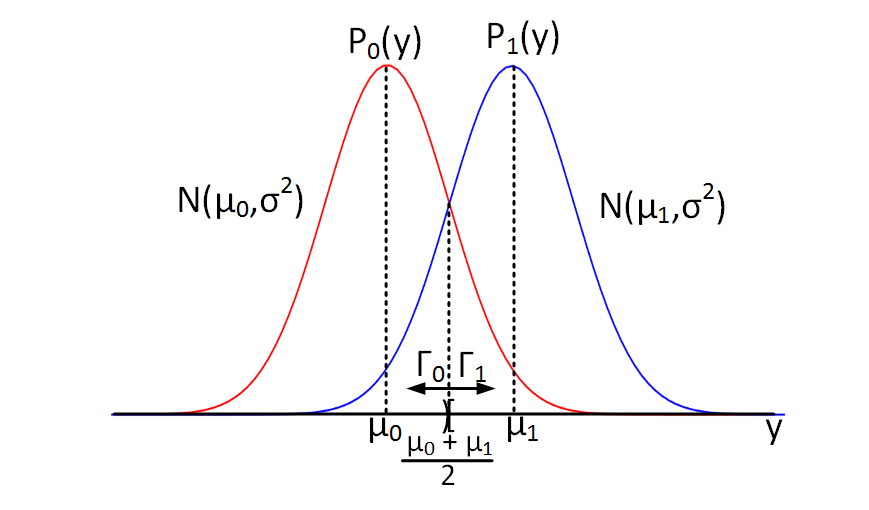
\includegraphics[scale=0.5]{Figures/Gaussian}
\caption{Illustration of location testing with Gaussian Error}
\label{fig:Gaussian}
\end{figure}
\begin{align*}
P_F(\delta_{NP}) &= \int_{y_0}^{\infty} f_{\mathcal{N}(\mu_0,\sigma^2)}(x) dx\\
&=1 - \int_{-\infty}^{y_0} f_{\mathcal{N}(\mu_0,\sigma^2)}(x) dx\\
&=1- \Phi(\frac{y_0-\mu_0}{\sigma}) ,\Phi \text{is standard normal cdf.}
\end{align*}
\begin{align*}
P_F(\delta_{NP}) &=
1 - \Phi(\frac{y_0-\mu_0}{\sigma}) = \alpha\\
 y_0 & = \sigma\Phi^{-1}(1-\alpha)+\mu_0
\end{align*}
The corresponding optimal detection probability is
\begin{align*}
P_D(\delta_{NP}) &= \int_{y_0}^{\infty} f_{\mathcal{N}(\mu_1,\sigma^2)}(x) dx\\
&=1 - \int_{-\infty}^{y_0} f_{\mathcal{N}(\mu_1,\sigma^2)}(x) dx\\
&=1- \Phi(\frac{y_0-\mu_1}{\sigma})\\
&=1-\Phi(\frac{\sigma\Phi^{-1}(1-\alpha)+\mu_0-\mu_1}{\sigma})\\
&=1-\Phi(\Phi^{-1}(1-\alpha)-d)\\[-20pt]
\end{align*}
\begin{align*}
{\text {where                                                                              } 
d := \frac{\mu_1-\mu_0}{\sigma} \text{ is signal to noise ratio(SNR).}}\\
\end{align*}
\begin{figure}[h]
\centering
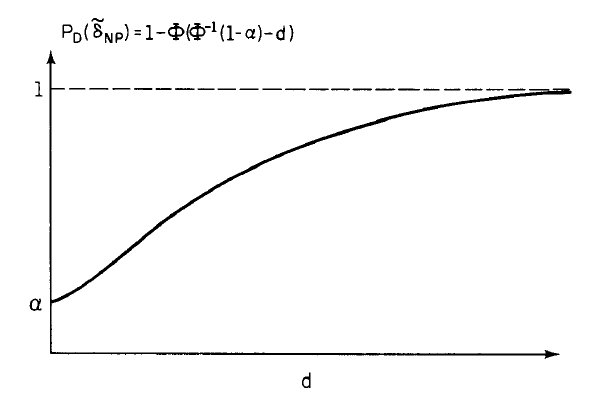
\includegraphics[scale=0.75]{Figures/Power}
\caption{$P_D$ vs d}
\label{fig:$P_D$ vs d}
\end{figure}
As d increases keeping $\alpha$ constant, $\Phi(\Phi^{-1}(1-\alpha)-d)$ decreases.
As a result $P_D(\delta_{NP})$ increases.\\
\begin{figure}[h]
\centering
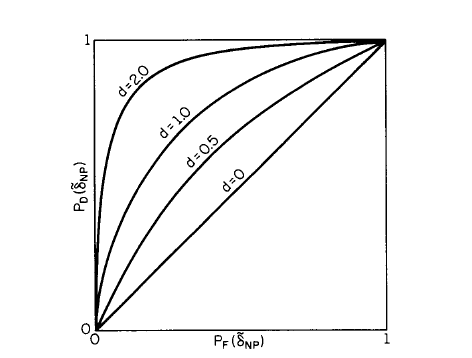
\includegraphics[scale=0.75]{Figures/ROC}
\caption{ROC}
\label{fig:ROC}
\end{figure}
At $\alpha$ = 0 and keeping d constant, $\Phi^{-1}$(1) = $\infty$ thus $P_D$ = 0.\\
At d = $\infty$ we can achieve the ideal conditions.\\ 
This curve between  $P_D(\delta_{NP})$ and $\alpha$ is called Receiver Operating Characteristic (ROC).\\
From the Neyman-Pearson lemma we can say that $P_D$ obtained from the ROC curve at a particular $\alpha$ and d is the best value that can be achieved,anything above this could not be obtained.\\[80pt]
{\bf Example 2: Neyman-Pearson testing for Binary Channel:}\\
For a binary channel $\Gamma$ = \{0,1\} and
Level $\alpha$ $\in$ [0,1] is given.\\[-10pt]
\begin{align*}
L(y) = P_1(y)/P_0(y) = \begin{cases}& (\frac{\lambda_1}{1-\lambda_0}) ; y=0\\
& (\frac{1-\lambda_1}{\lambda_0}) ; y=1\\
\end{cases}
\end{align*}
\begin{figure}[h]
\centering
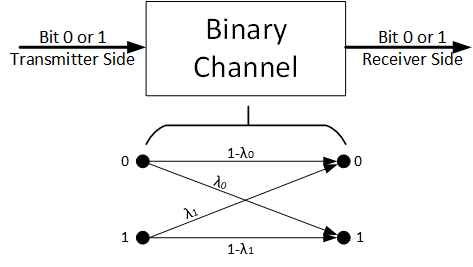
\includegraphics[scale=0.9]{Figures/BinaryChannel}
\caption{BinaryChannel}
\label{fig:binarychannel}
\end{figure}
In this case $\mathbb{P}$(L(y)=$\eta_0$) $\ne$ 0\\ 
In ideal case $\lambda_1$, $\lambda_0$ must be zero.\\
For concretness, let us assume that  $\lambda_1$, $\lambda_0$ $>$ 0 and $\lambda_1$+$\lambda_0$ $<$ 1.\\
This is equivalent to saying 
\begin{align*}
\frac{\lambda_1}{1-\lambda_0} < \frac{1-\lambda_1}{\lambda_0}\\
\end{align*}
As we saw the Neyman-Pearson rule must have the form\\
\begin{align*}
 \delta_{NP}(y) = \begin{cases}
1, &  \text{if }P_1(y)/P_0(y)>\eta_0 \\
\gamma_0, & \text{if }P_1(y)/P_0(y)=\eta_0\\
0, &  \text{if }P_1(y)/P_0(y) < \eta_0 \\
\end{cases} 
\end{align*}
\begin{figure}[h]
\centering
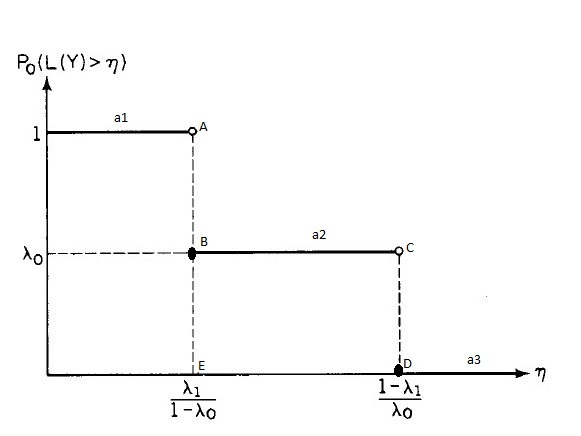
\includegraphics[scale=0.75]{Figures/img}
\label{fig}
\end{figure}
To solve this problem it is enough to set $\eta_0$.\\
From previous class we know that
\begin{align*}
\eta_0 := min \{ \eta \geq 0 : \mathbb{P}[L(y)>\eta] \leq \alpha\} \\
\end{align*}
Thus, the choice of likelihood ratio threshold is:\\
\begin{align*}
\eta_0=\left\{
\begin{array}{cc}
\frac{1-\lambda_1}{\lambda_0}  &,  0\leq\alpha\leq\lambda_0\\
\frac{\lambda_1}{1-\lambda_0}  &,  \lambda_0\leq\alpha\leq1\\
0 &, \alpha=1
\end{array}\right.
\end{align*}
And the randomization  probability $\gamma_0$ is\\
\begin{align*}
\gamma_0=\left\{
\begin{array}{cc}
\frac{\alpha}{\lambda_0}  &, 0\leq\alpha\leq\lambda_0\\
\frac{\alpha-\lambda_0}{1-\lambda_0}  &, \lambda_0\leq\alpha<1\\
\text{arbitrary} &, \alpha=1
\end{array}\right.
\end{align*}
Here, the possible $\eta$ values i.e $\frac{\lambda_1}{1-\lambda_0}$ and $\frac{\lambda_1}{1-\lambda_0}$ are strictly positive. Hence, $\eta_0$ is also positive.\\
So, the N-P rule:\\ If 0$\leq\alpha\leq\lambda_0$\\[-10pt]
\begin{align*}
\delta_{NP}(y)=\left\{
\begin{array}{cc}
0 &, y=0\\
\frac{\alpha}{\lambda_0} &,y=1
\end{array}\right.
\end{align*}
If $\lambda_0\leq\alpha\leq1$:\\[-10pt]
\begin{align*}
\delta_{NP}(y)=\left\{
\begin{array}{cc}
\frac{\alpha-\lambda_0}{1-\lambda_0} &, y=0\\
1 &, y=1
\end{array}\right.
\end{align*}
ROC for the binary channel : $(\lambda_0+\lambda_1<1)$\\
$\mathbb{P}_D[\delta_{NP}]$ in the first case $0\leq\alpha<\lambda_0$ has only one term as in this case probabitlity of choosing y=1 is 0 when y=0 is observed.Thus $\mathbb{P}_D[\delta_{NP}]$ is the product of probability of transmitting 1 i.e $(1-\lambda_1)$ and probability of deciding 1 when y=1 is observed i.e $(\frac{\alpha}{\lambda_0}).$\\
Similarly when $\lambda_0\leq\alpha\leq1$ $\mathbb{P}_D[\delta_{NP}]$ has two terms. First case is when 1 is transmitted, 1 is received and 1 is decided. Probability for this is  ${1-\lambda_1}$. The second term is when 1 is transmitted, 0 is received but 1 is decided. Probability for this is product of ${\lambda_1}$(probalilty of 0 received when 1 transmitted) and $\frac{\alpha-\lambda_0}{1-\lambda_0}$.
\begin{align*}
\mathbb{P}_D[\delta_{NP}]=\left\{
\begin{array}{cc}
(1-\lambda_1)\frac{\alpha}{\lambda_0} &, 0\leq\alpha<\lambda_0\\
\frac{\lambda_1(\alpha-\lambda_0)}{1-\lambda_0}+(1-\lambda_1) &, \lambda_0\leq\alpha\leq1
\end{array}\right.
\end{align*}
When $\lambda_1$=0 and $\lambda_0$=0, then, $\mathbb{P}(\delta_{NP})=1$ for all $\alpha$. $\Rightarrow$ "Ideal rule".\\
\begin{figure}[h]
\centering
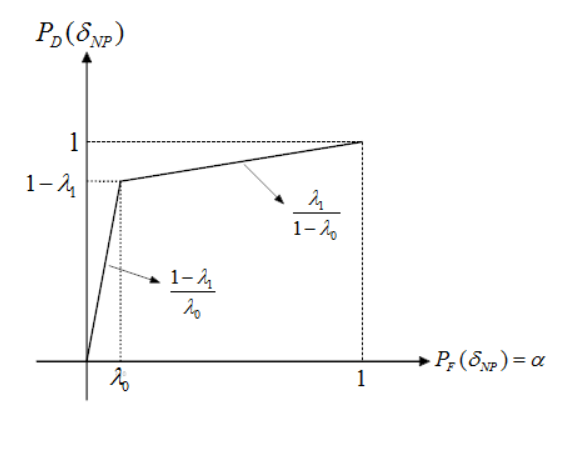
\includegraphics[scale=0.75]{Figures/plot1_snip}
\caption{$\mathbb{P}_D(\delta_{NP})$ vs $\mathbb{P}_F(\delta_{NP})$}
\end{figure}
Note that as $\frac{1-\lambda_1}{\lambda_0}>\frac{\lambda_1}{1-\lambda_0}$
the slope of the first part of the curve is larger than that of the slope of the second part.Thus in the ideal case is a jump from 0 to 1 at origin.\\
\section{Composite Hypothesis Testing}
Composite hypothesis testing generalizes "Simple" hypothesis testing. It answers the problem of analyzing hypothesis testing problems with more than one generating probability distributions per hypothesis.\\[50pt]
{\bf Simple hypothesis testing:} \\
$H_0$ : $Y$  $\sim$ $\mathbb{P}_0$\\
$H_1$ : $Y$  $\sim$ $\mathbb{P}_1$ \\
For each of the hypothesis only a single probability distribution is defined over $\Gamma$.\\
But, in general many distributions could be active over $\Gamma$ for a particular hypothesis .\\
So, using Composite hypothesis testing we can analyze problems with more than one distribution defined per hypothesis.\\[10pt]
\textbf{Example:}\\
$H_0$: "No enemy aircraft in the vicinity"\\
$H_1$: "Enemy aircraft is at a distance $x$ ", $x$$\in$[0,$x_{max}$]\\
\begin{figure}[h]
\centering
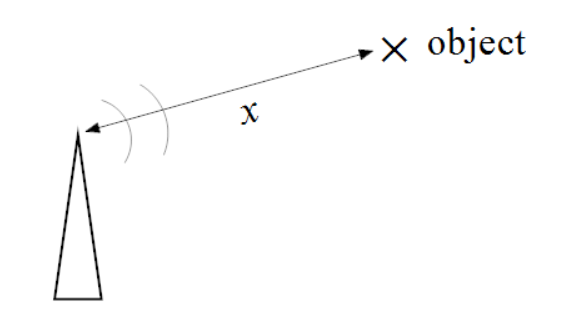
\includegraphics[scale=0.5]{Figures/radfig_snip}
\end{figure}
Depending on $x$ and some other parameters we may transmit different signals . \\
$\therefore$ Actual distribution over $\Gamma$ depends on the position of the aircraft.\\
\begin{figure}[h]
\centering
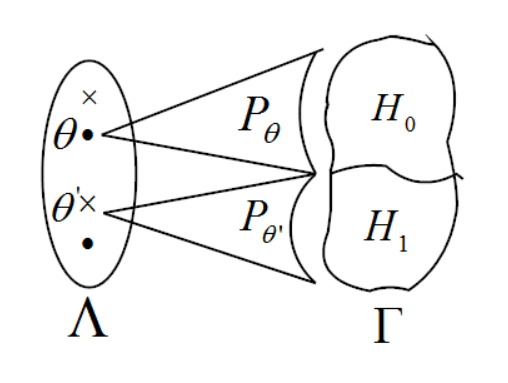
\includegraphics[scale=0.75]{Figures/fig2_snipp}
\caption{$\theta\sim\mathbb{P}_{\theta}$ and $\theta'\sim\mathbb{P}_{\theta'}$ }
\end{figure}
\begin{align*}
\Gamma&: \text{Observation space}\\
\wedge&: \text{Parameter space}\\[-10pt]
\end{align*}
\textbf{Example:} For a simple hypothesis $\wedge$=\{0,1\}\\[-15pt]
\subsubsection{Bayesian composite hypothesis testing:}
\textbf{Bayesian assumption:} The parameter $\Theta$ is drawn from $\wedge$ according to prior 
distribution $\pi$ on $\wedge$.\\[10pt]
{\bf Note:}\\
In Composite hypothesis testing, there are only two hypothesis  $H_0$ and $H_1$. But, each hypothesis has more than one possible distributions over $\Gamma$.\\
Where as in a Simple hypothesis testing $H_0$ and $H_1$ have a single probability distribution $\mathbb{P}_0$ and $\mathbb{P}_1$ resp defined over $\Gamma$.\\[10pt]
{\bf Costs:}\\ $C(i,\theta)$: A cost for declaring hypothesis $H_i$ when the true distribution is $\mathbb{P}_{\theta}$\\$\forall$ i$\in$\{0,1\} ,$\forall \theta\in\wedge$\\[10pt]
{\bf Motivation to decide costs $C(i,\theta)$:} \\
In the example of radar we could model costs which depend on $\theta$ where $\theta$ could be seen as the distance x from the enemy aircraft. Thus the probability of missed detection of the enemy aircrafts at shorter distances could be made smaller than those at longer distances as we don't want to miss the detection of a "nearby" aircraft. \\[10pt]
\textbf{Decision rule:} $\delta: \Gamma\rightarrow\{0,1\}$\\[10pt]
\textbf{Conditional risks:}
$\forall\theta\in\wedge$ the conditional risk of $\delta$ for generating $\mathbb{P}_{\theta}$ is defined to be
\begin{align*}
\mathbb{E}_{\theta}[C(\delta(Y),\theta)]:=R_\theta(\delta)\\
\end{align*}
\textbf{Bayes risk:} The Bayes risk of $\delta$ is :
\begin{align*}
r(\delta)&=\mathbb{E}[R_{\Theta}(\delta)]\\
\Theta&\sim\pi  \text{ on }  \wedge
\end{align*}

\end{document}